\documentclass{article}
\usepackage{ctex}
\usepackage{graphicx}
\title{AUC 学习笔记}
\author{Li Zhenyang}
\date{October 2019}
\email{lizhenyang\_2008@163.com}
\begin{document}
   \maketitle
   \section{AUC 是什么?}
   \section{举个例子}
   \section{计算代码}
   \section{一些思考}
   根据 [模型评估指标AUC(area under the curve)](https://blog.csdn.net/liweibin1994/article/details/79462554) 这个文章里面的一个图,AUC 可以被认为是正负样本分布的重合程度。重合程度越高,AUC 越大。当正负样本分布较接近时,AUC 接近 0.5。
   \begin{figure}[h]
       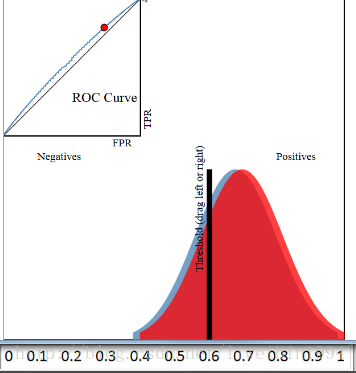
\includegraphics[width=0.8\textwidth]{auc-and-distribution.png}
       \label{auc-and-distribution}
       \caption{auc-and-distribution}
   \end{figure}


   参考图 \ref{auc-and-distribution},AUC 其实就是竖线右边的部分占篮红区域的比例。

\end{document}
